\documentclass[12pt]{article}
%\usepackage{times}
\usepackage{cite}
\usepackage{graphicx}
\usepackage{url}
\setlength{\parskip}{1em}
\setlength{\parindent}{0em}
%this is a comment
\title{CS 361 \\ Software Design Specification and User Interface (SDSUI): \\ Digital Ghostwriter}
\author{Thomas Hollenberg (hollenbt), Zachary Thomas (thomasza),\\ Amar Raad (raadv), Jared Tence (tencej), \\  Zech DeCleene (decleenz)}
\date{February 2nd, 2018}

\begin{document}
\maketitle
\newpage
\tableofcontents

\newpage

\section{User Interface Prototypes}

\begin{figure}[ht]
  \centering
    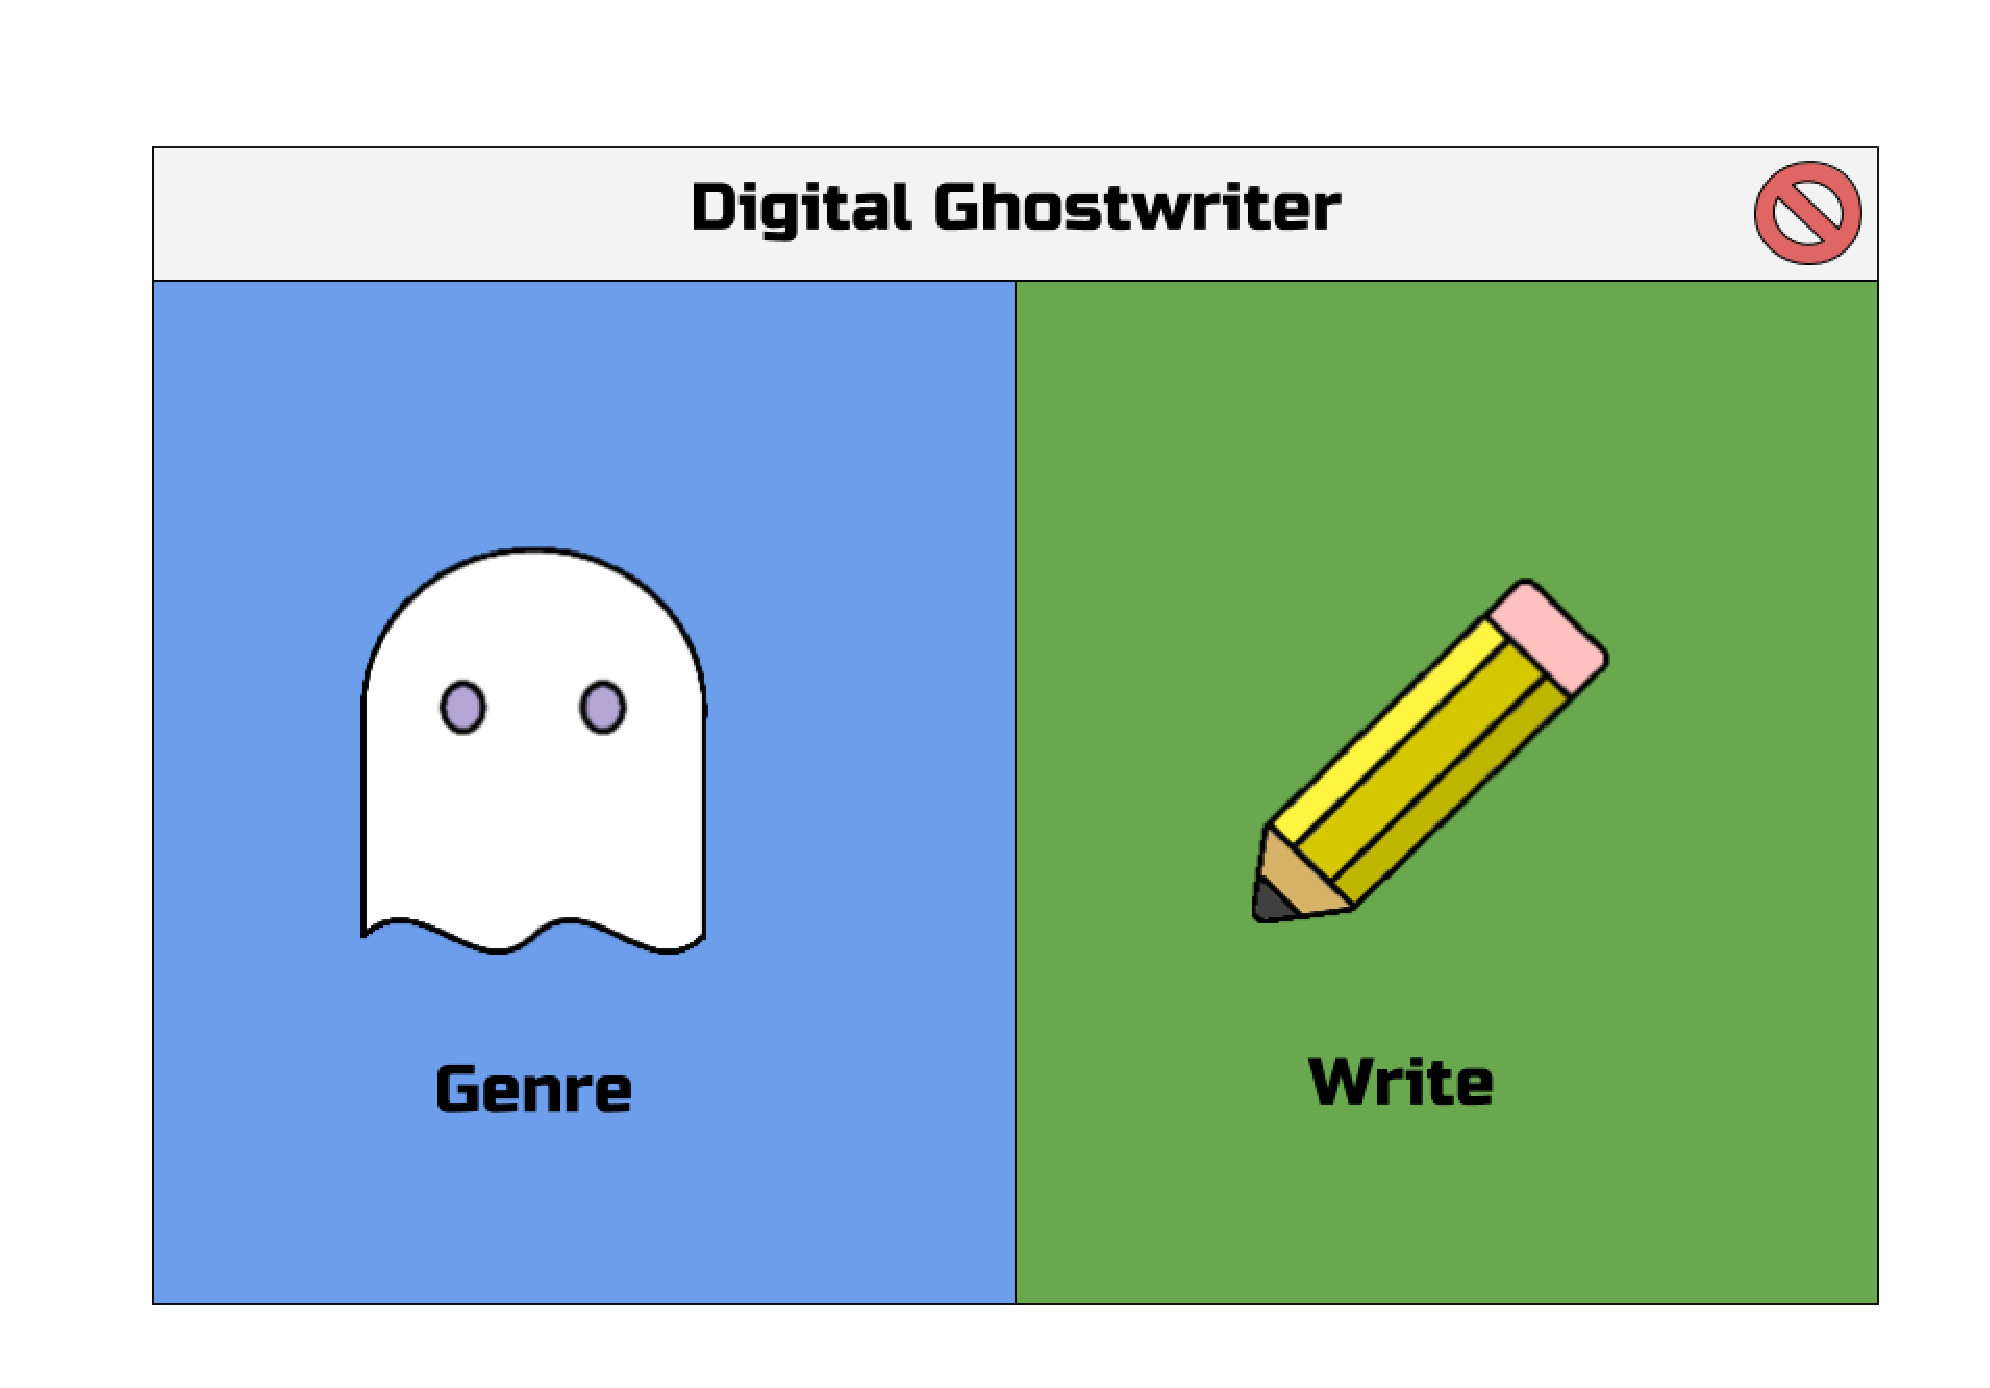
\includegraphics[scale=0.5]{GW.eps}
    \caption{Main menu.}
\end{figure}

This is the start screen for Digital Ghostwriter.
Users can select "Genre" or "Write" by clicking either side of the screen.

In the task-bar at the top of screen the red icon gives the user the option to exit the program.

\newpage

\begin{figure}[ht]
  \centering
    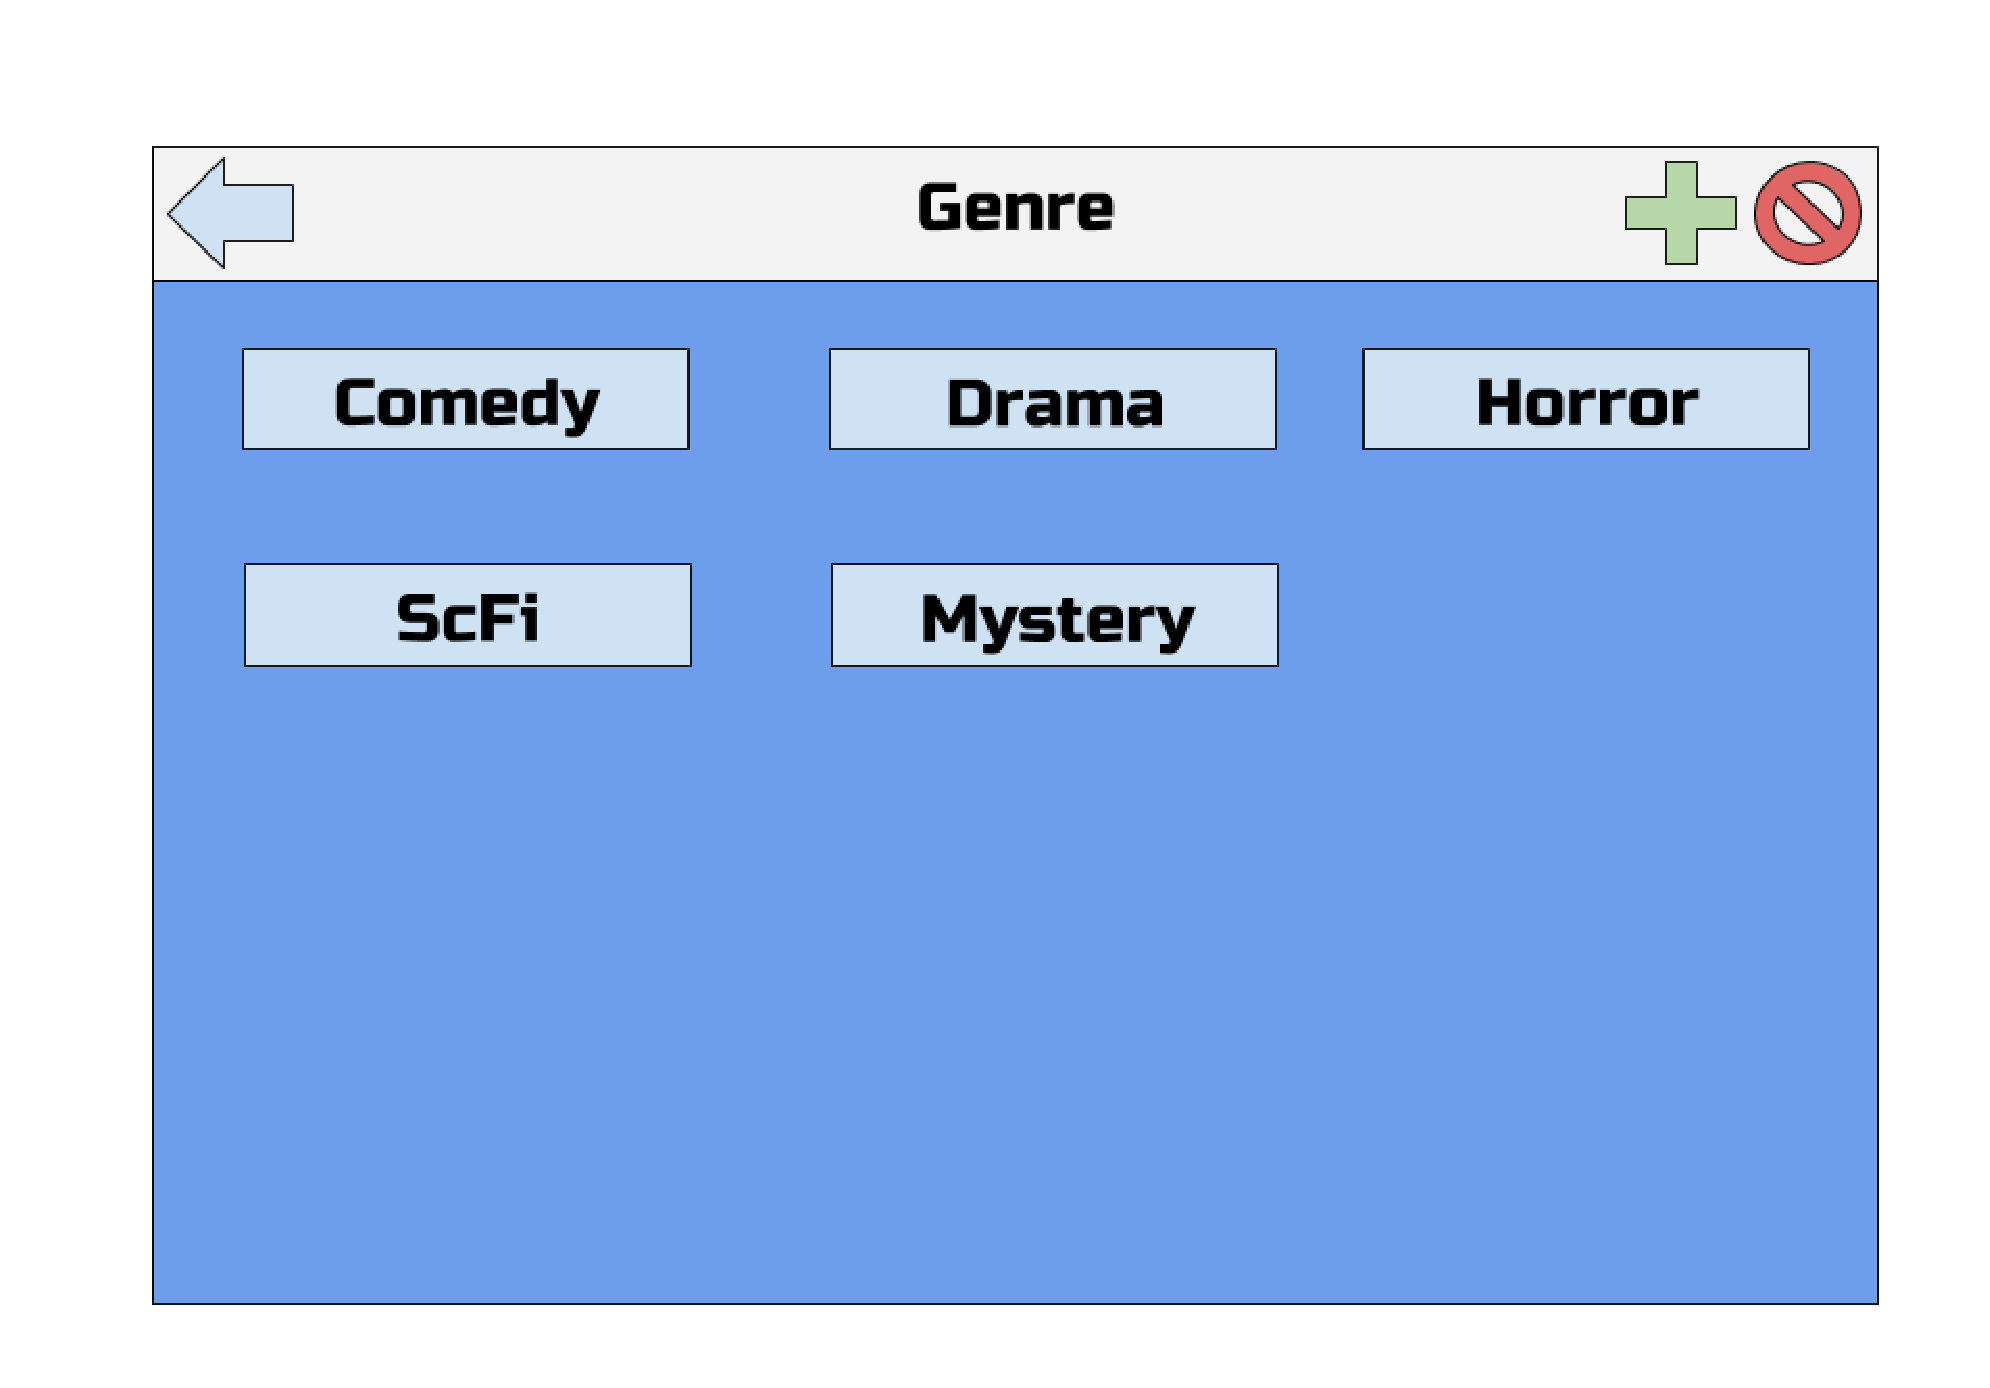
\includegraphics[scale=0.5]{G1.eps}
    \caption{Genre menu.}
\end{figure}

If the user selected "Genre" on the main menu this is the screen they will be met with. Clicking on a specific genre brings them to a different screen that displays the files used to train Digital Ghostwriter about that genre. 

The task-bar now has an arrow icon that allows the user to go to the previous screen, and a plus icon that allows the user to add a new genre.

\newpage

\begin{figure}[ht]
  \centering
    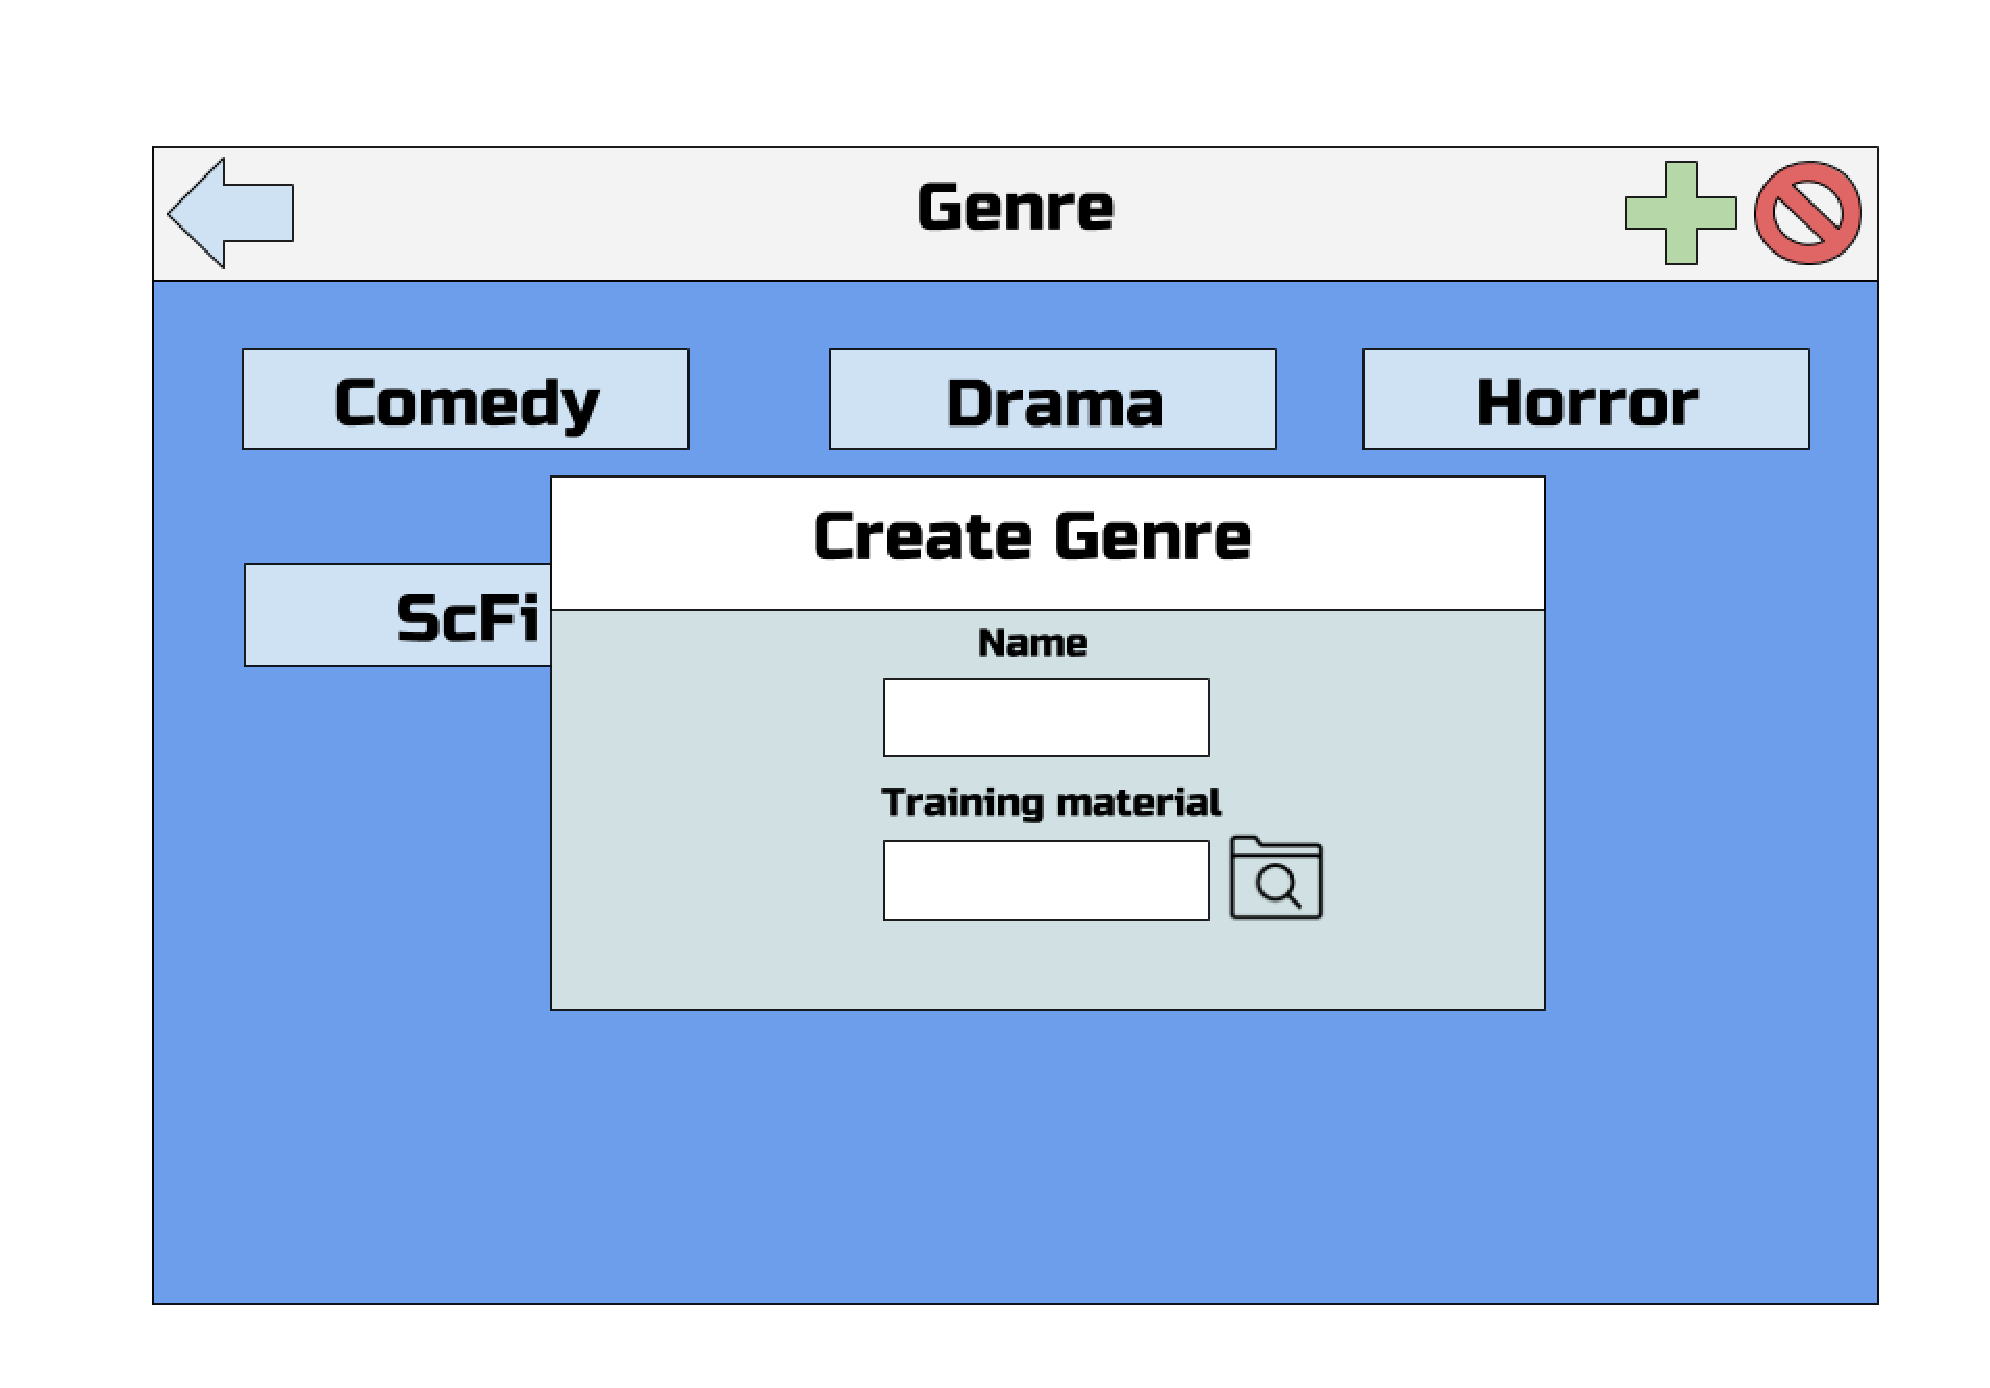
\includegraphics[scale=0.5]{G3.eps}
    \caption{Genre menu pop-up.}
\end{figure}

In this scenario the user has clicked on the green icon in the task-bar and is now met with a pop-up screen. The user must enter a name for the genre they wish to create and also a path to a folder filed with documents that Digital Ghostwriter can use to train and understand this new genre. \newline \textbf{(Use case 2)}

\newpage

\begin{figure}[ht]
  \centering
    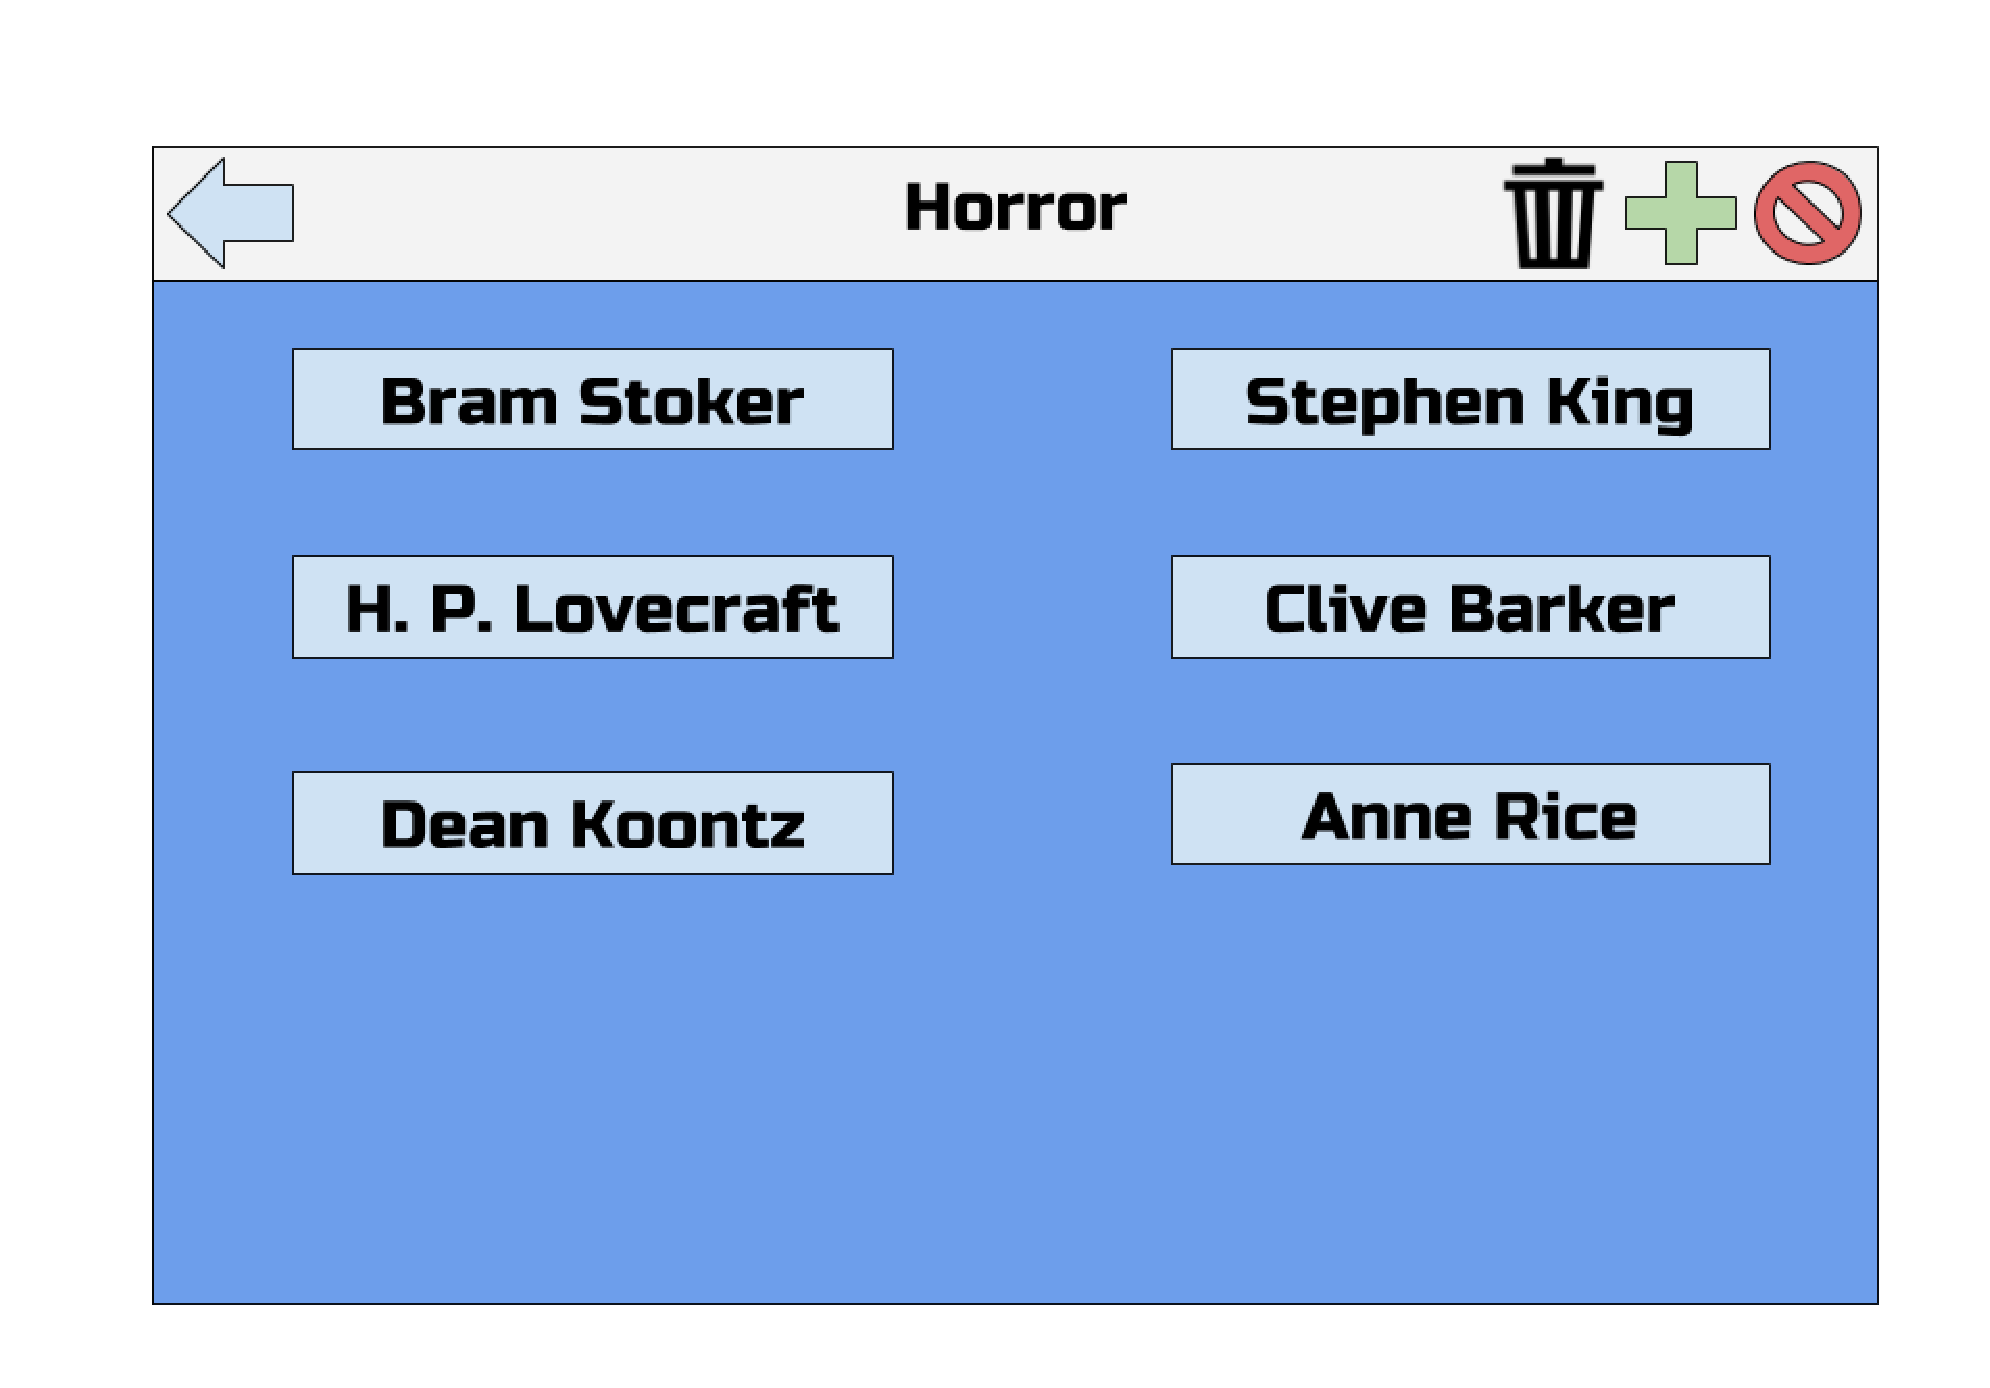
\includegraphics[scale=0.5]{G2.eps}
    \caption{Genre menu pop-up.}
\end{figure}

The user has selected the "Horror" genre from the previous screen and are now met with all the files (in this case Authors) that were used to train Digital Ghostwriter about the horror genre. The user may selected a file by clicking on it giving them a prompt to delete it and have Digital Ghostwriter unlearn the material. \newline \textbf{(Use case 3)}

There is now a new icon in the task-bar, the trashcan icon gives the user the option to delete the "Horror" genre. The green icon now gives the user the option to add a file to this genre that Digital Ghostwriter will begin training with.

\newpage

\begin{figure}[ht]
  \centering
    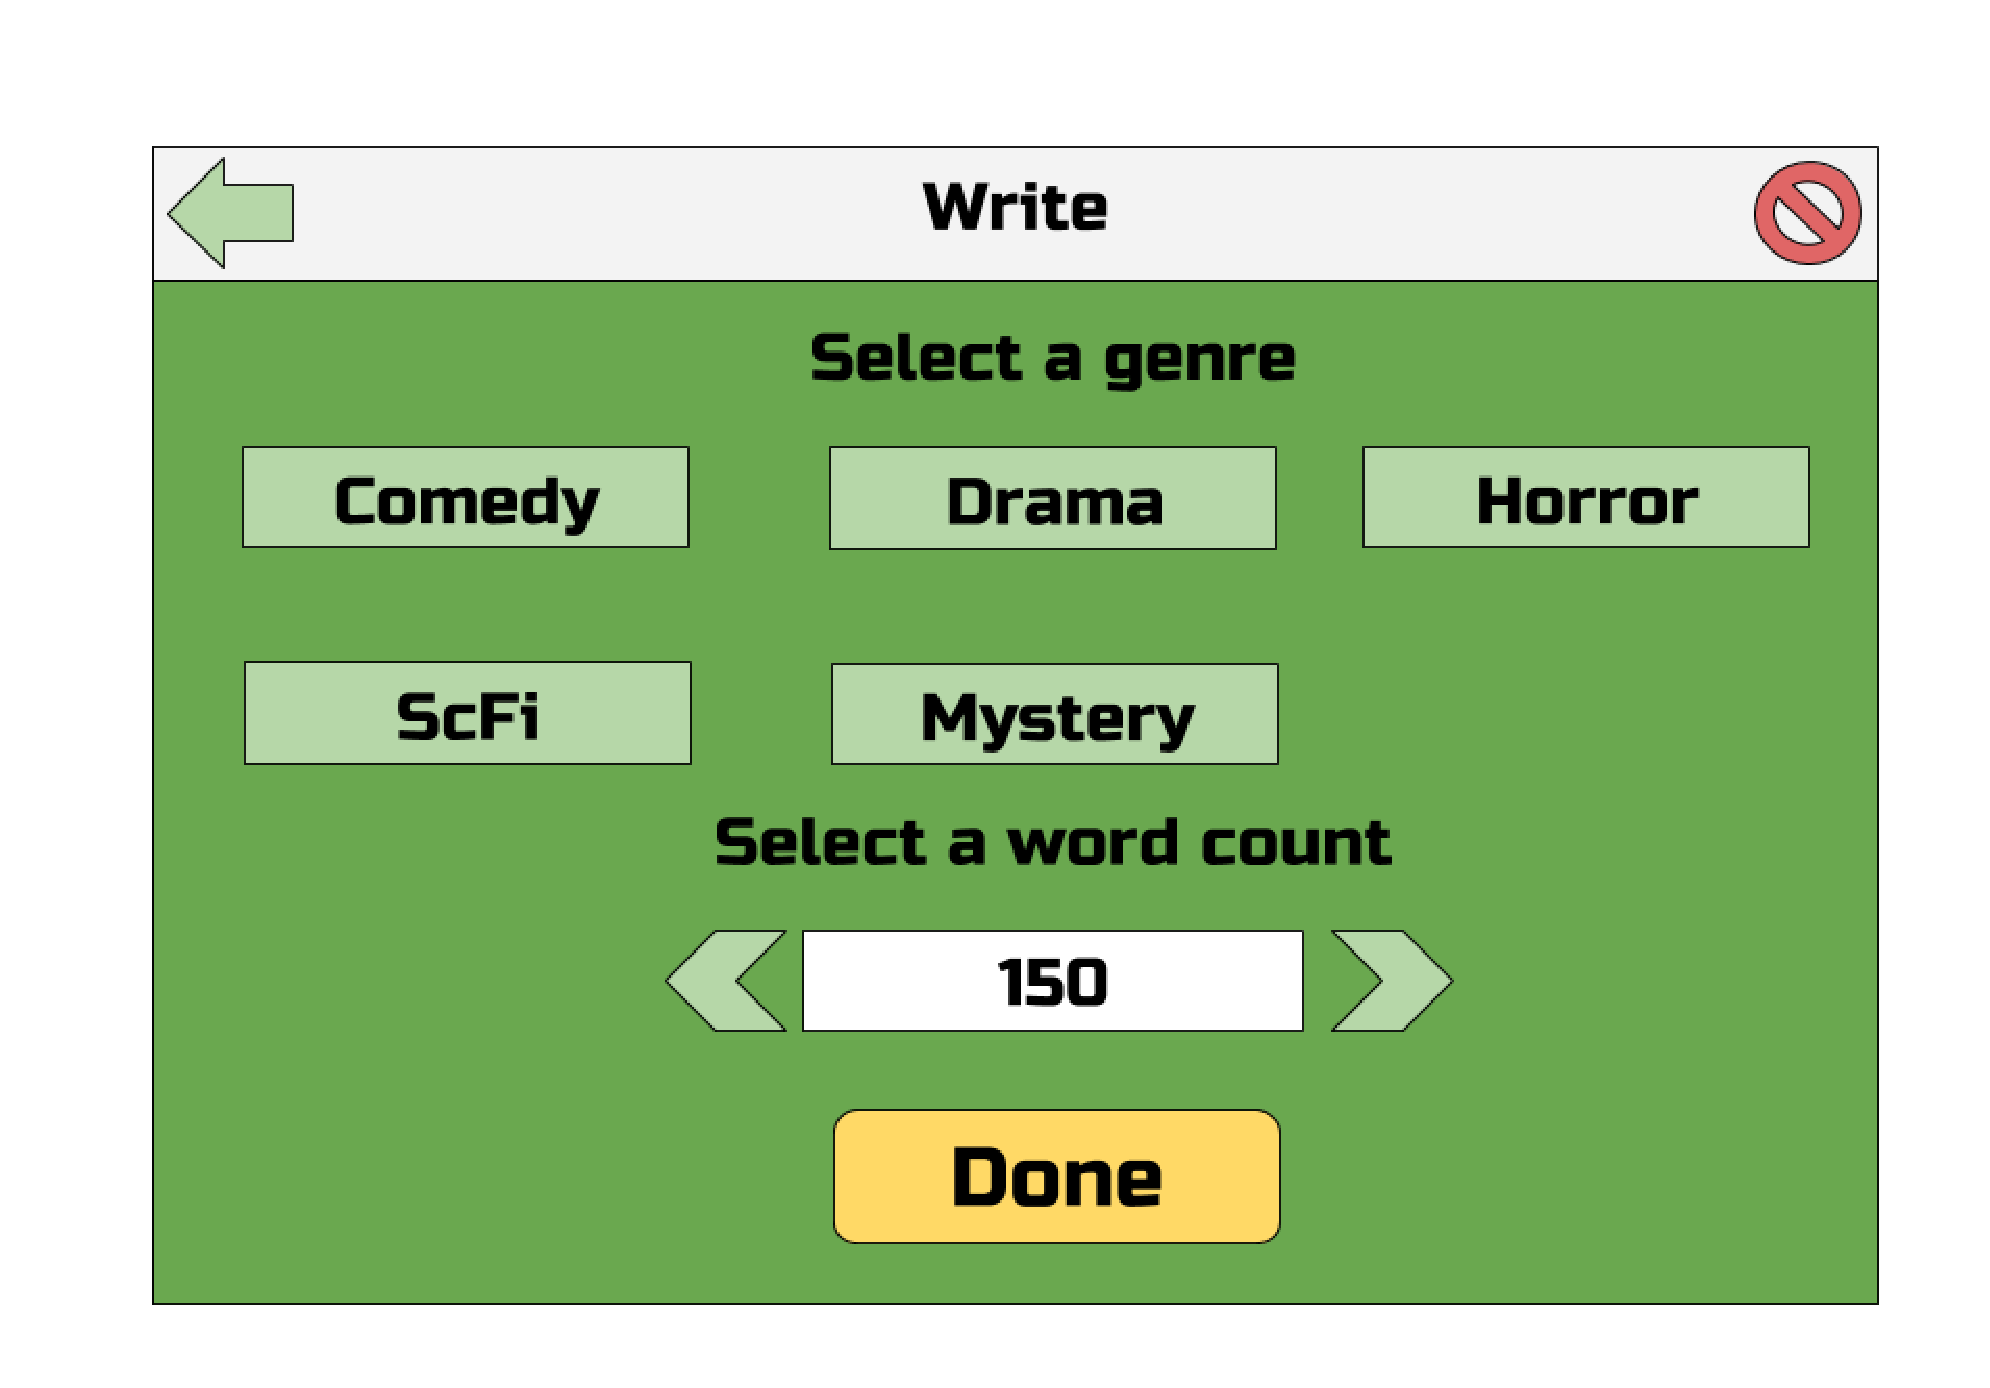
\includegraphics[scale=0.5]{W1.eps}
    \caption{Write menu.}
\end{figure}

If the user selected "Write" on the main menu this is the screen they will be met with. The user must select a genre and a word count for the document that Digital Ghostwriter is about to write. When they are satisfied with their selections they must click the "Done" button.

The task-bar has the same functionality that it has had on previous screens.

\newpage

\begin{figure}[ht]
  \centering
    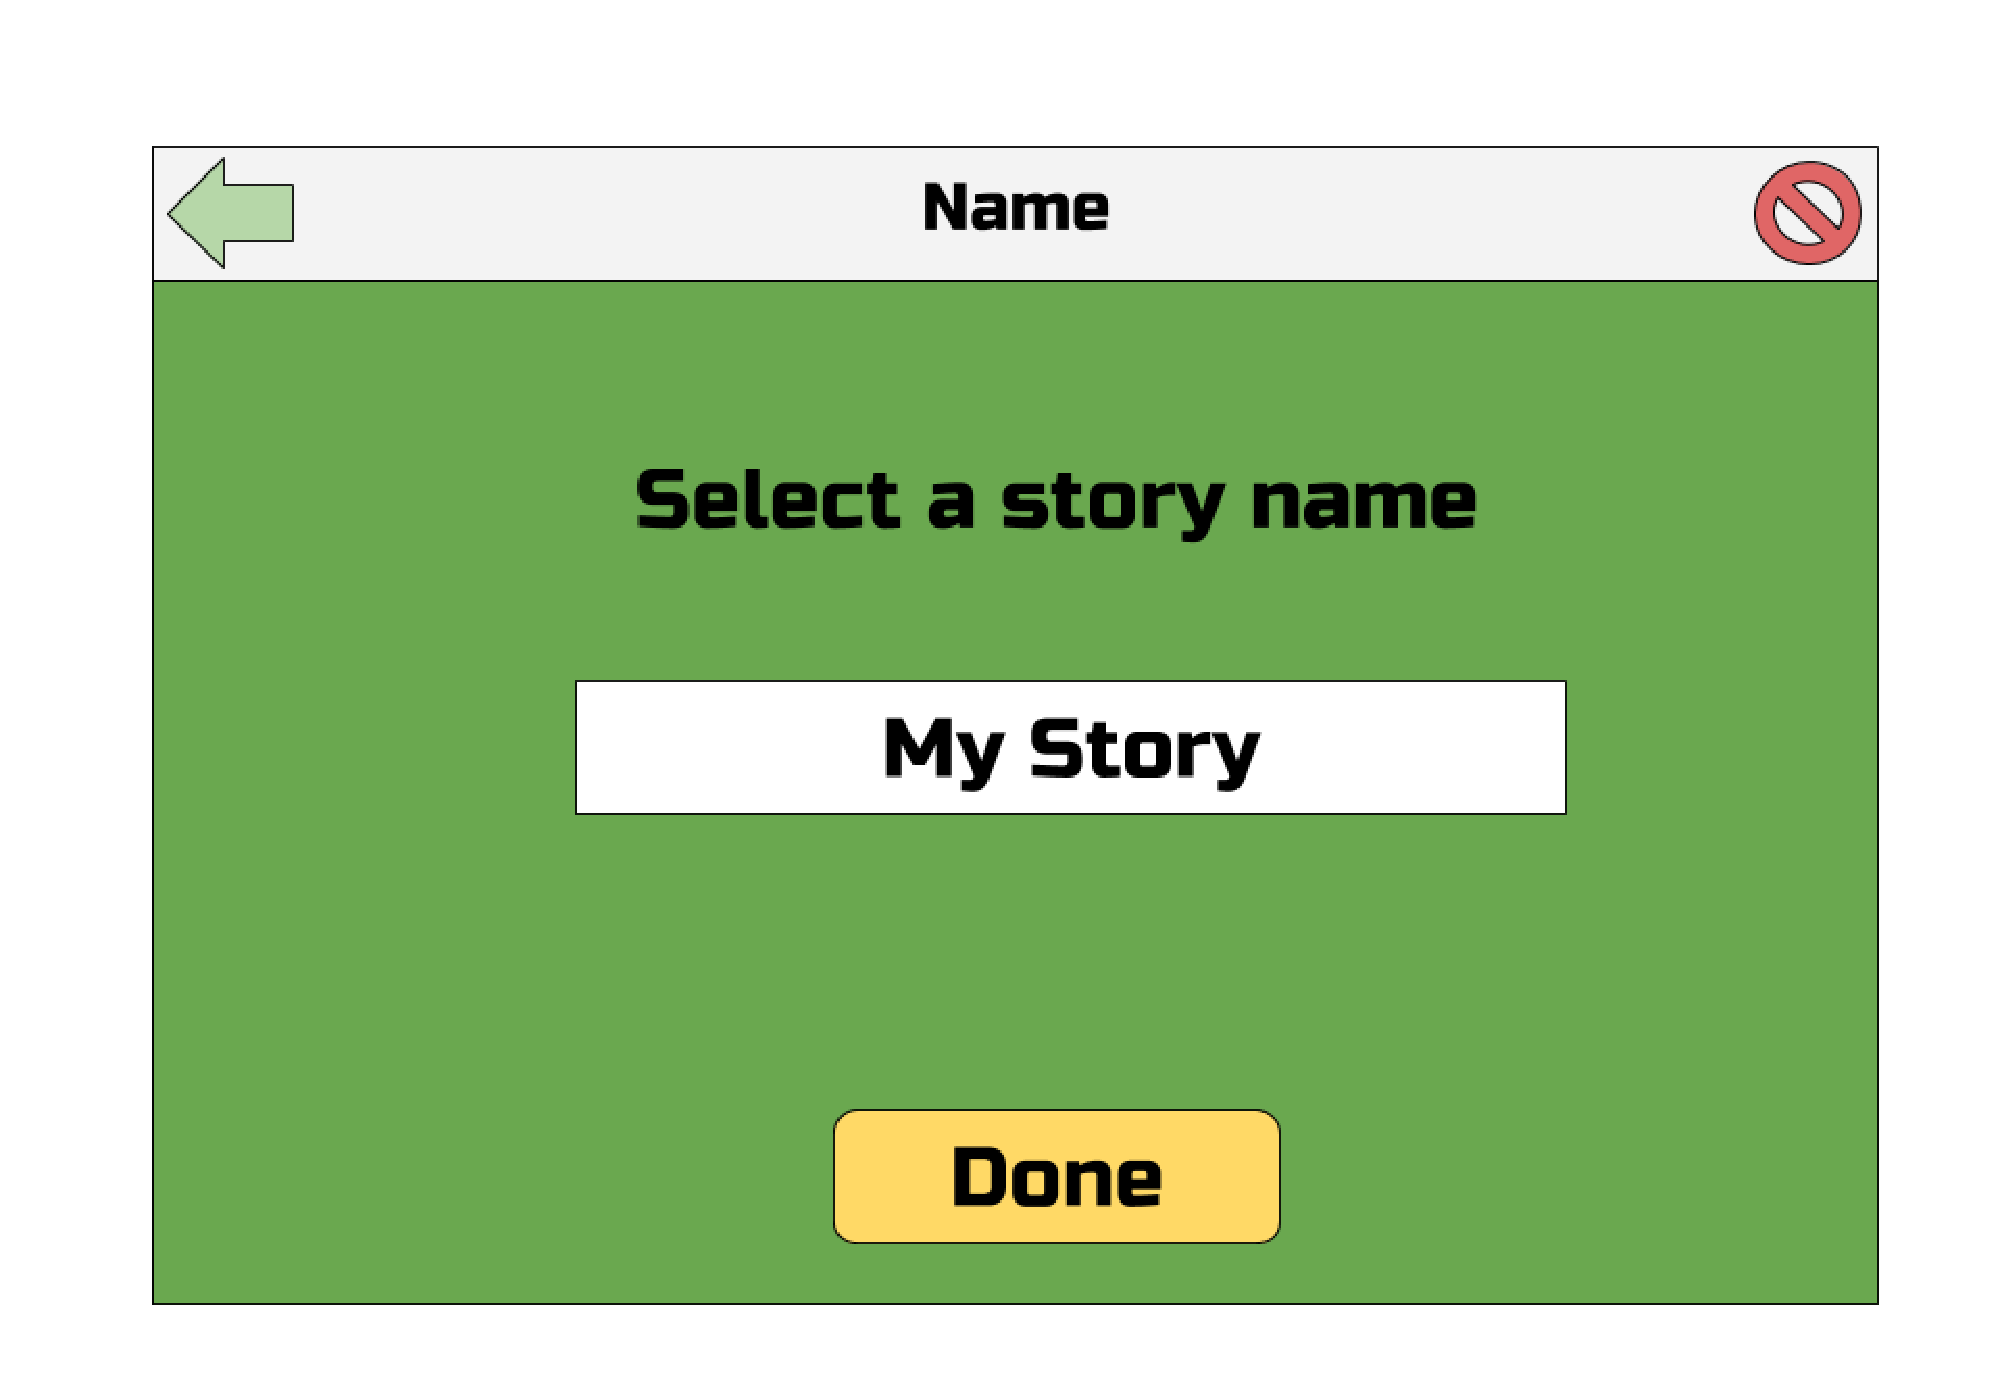
\includegraphics[scale=0.5]{W2.eps}
    \caption{Name file.}
\end{figure}

Here the user must select a name for the document that Digital Ghostwriter is about to write. When they have selected a name they must click the "Done" button to proceed.

\newpage

\begin{figure}[ht]
  \centering
    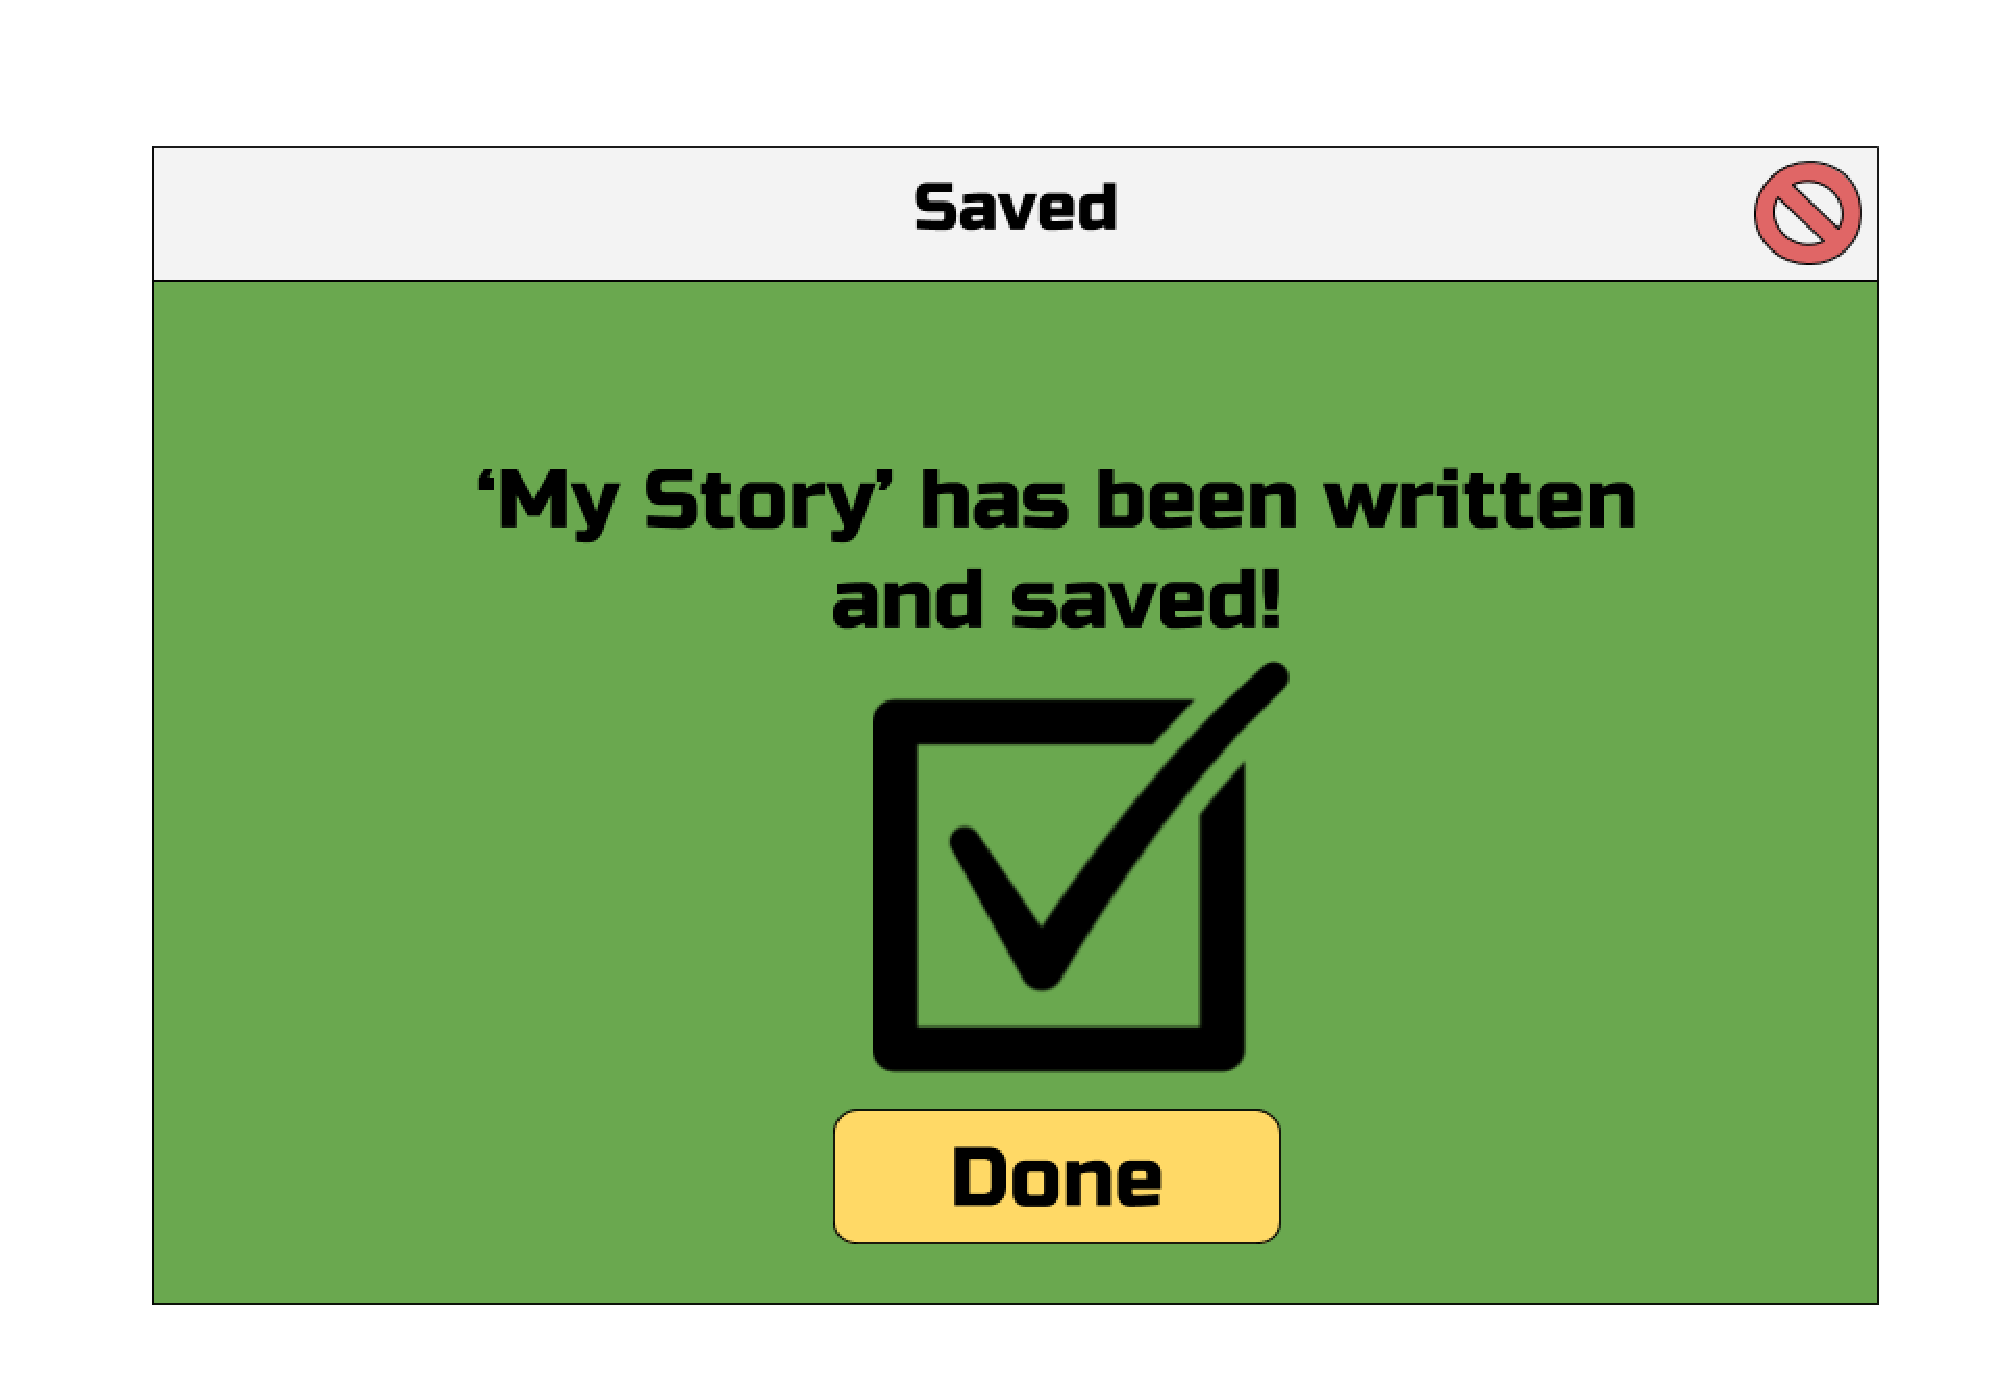
\includegraphics[scale=0.5]{W3.eps}
    \caption{File written.}
\end{figure}

After the user has selected all of the document settings and selected a name this screen is shown, indicating that Digital Ghostwriter has written and saved their document under the name they have given. Clicking the "Done" button at this point returns the user to the main menu. \newline \textbf{(Use case 1)}

\newpage 

\section{Class Diagram}
\begin{figure}[ht]
  \centering
    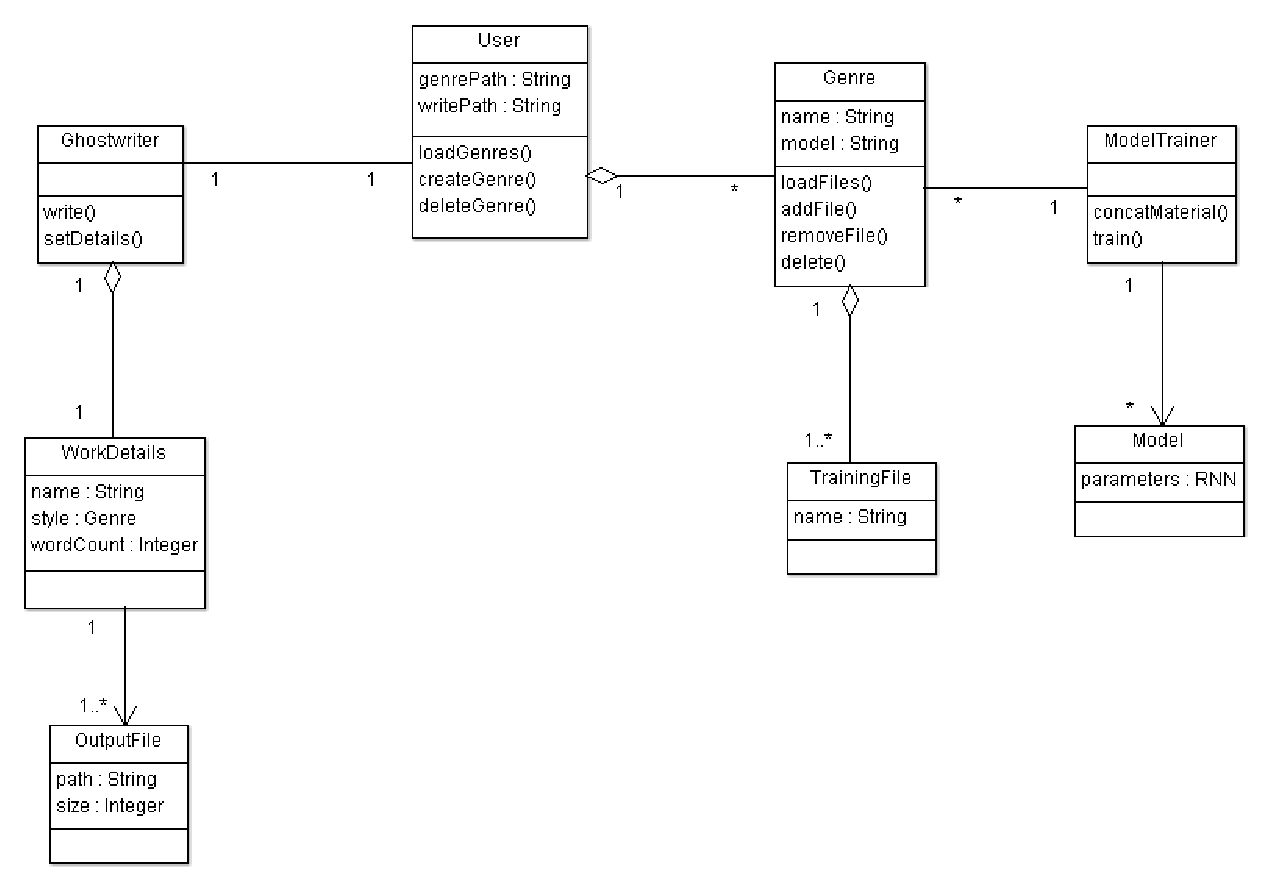
\includegraphics[scale=0.7]{ClassDiagram.eps}
\end{figure}

\newpage

\section{Sequence Diagrams}

\subsection{Create Short Story}
Generate a short story matching the users desired settings.
\begin{figure}[ht]
  \centering
    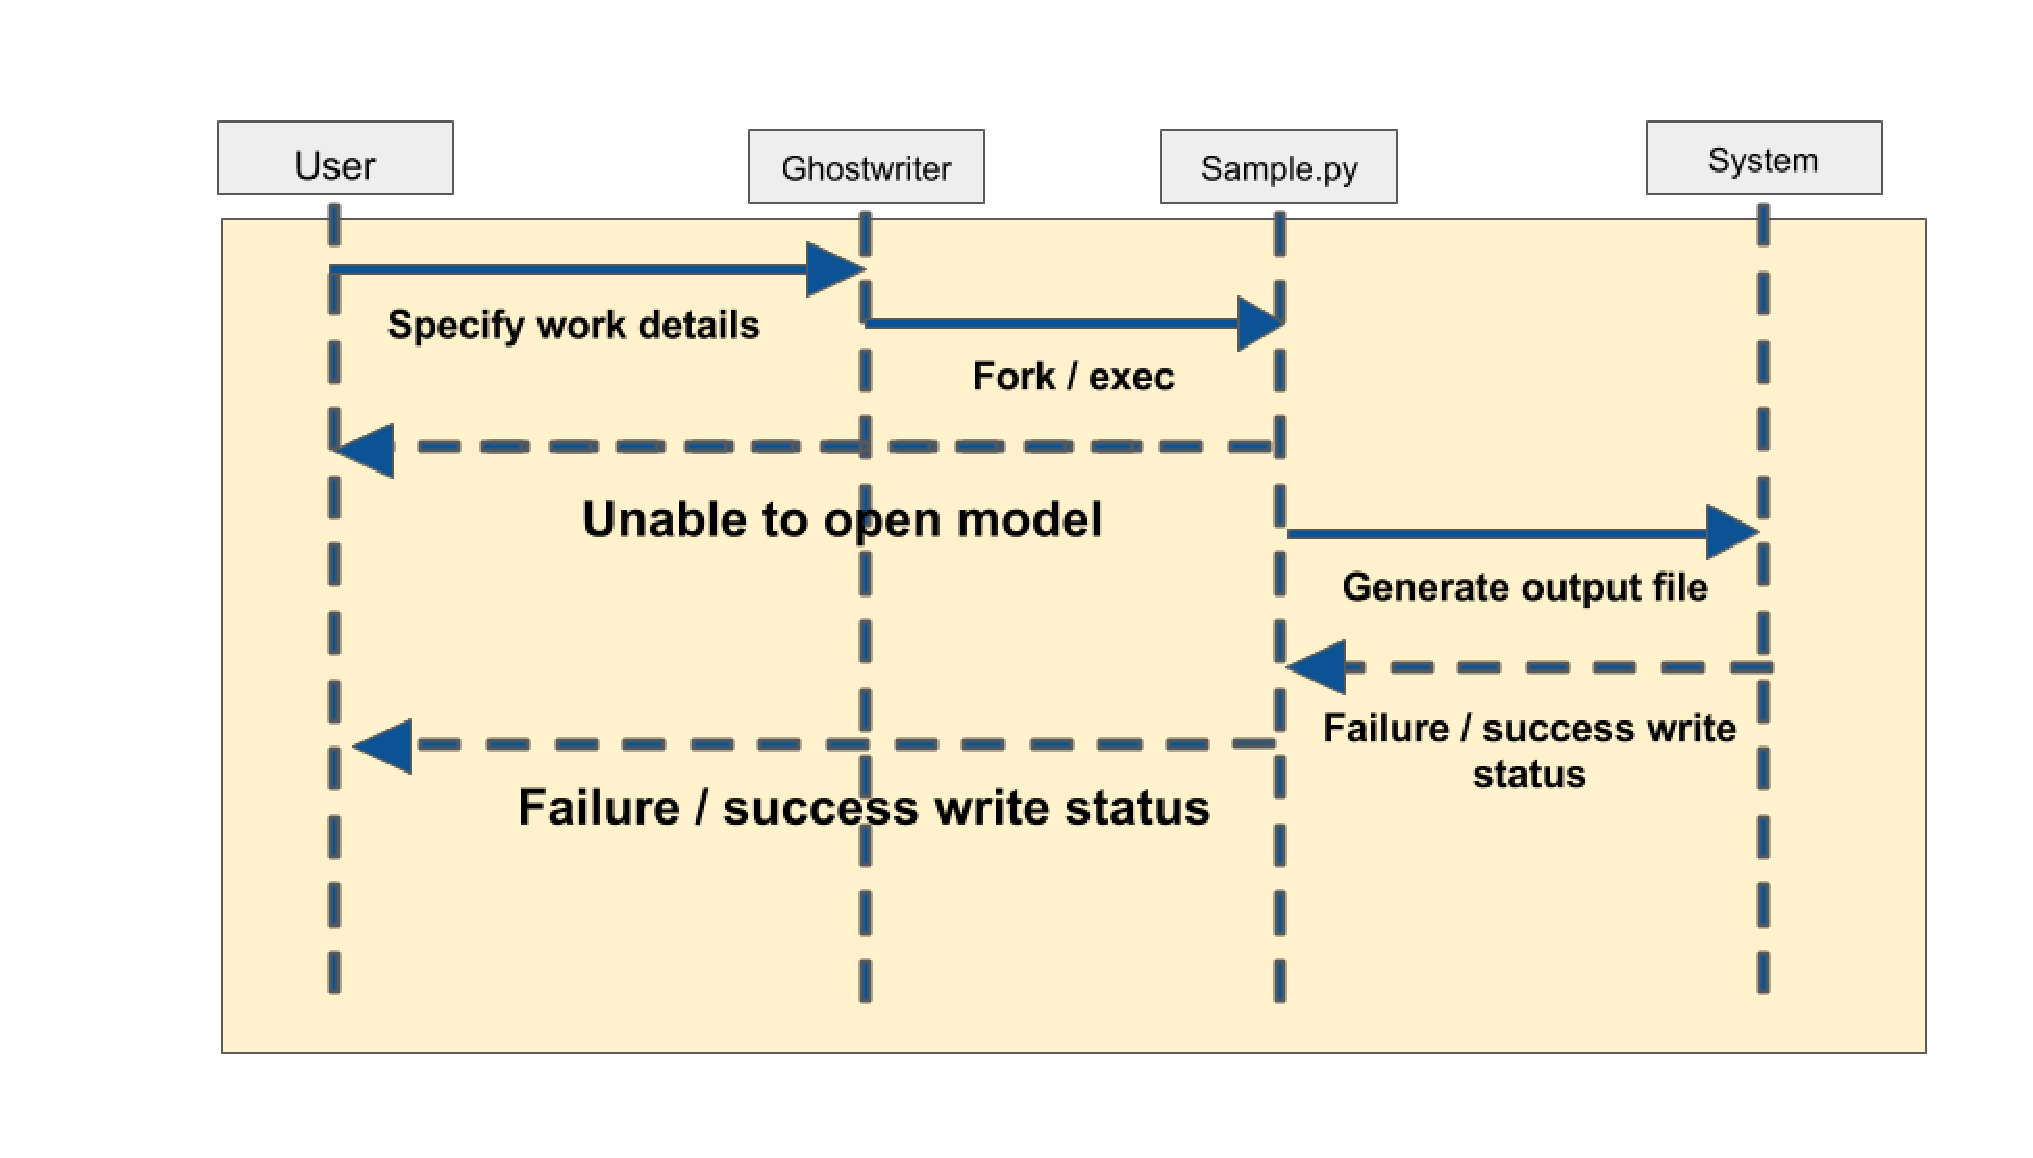
\includegraphics[scale=0.5]{Case1.eps}
\end{figure}

\newpage

\subsection{New Genre Creation}
Generate a new genre using text documents submitted by the user.
\begin{figure}[ht]
  \centering
    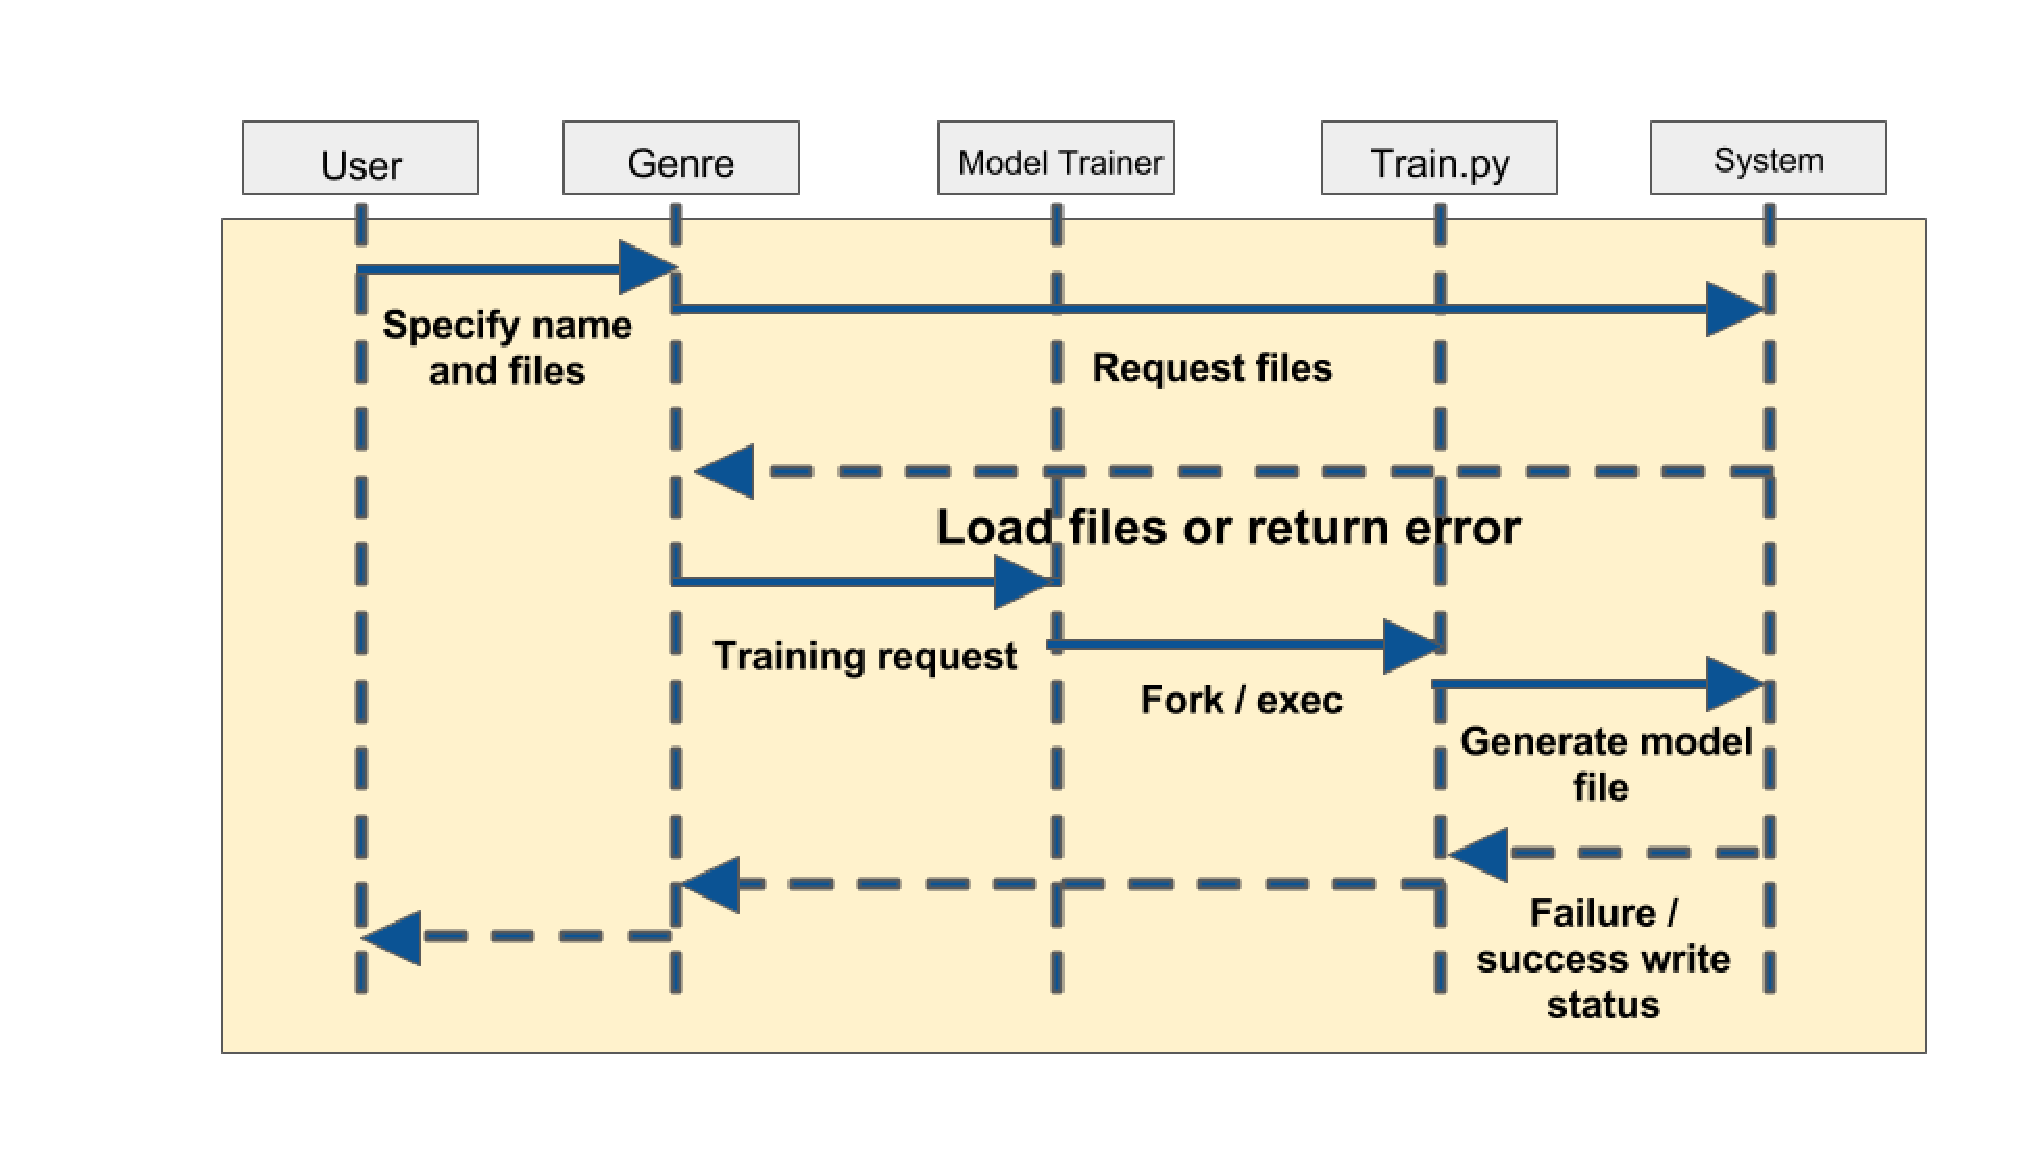
\includegraphics[scale=0.5]{Case2.eps}
\end{figure}

\newpage 

\subsection{View Authors}
Allows users to see what authors works are being used in a specific genre.
\begin{figure}[ht]
  \centering
    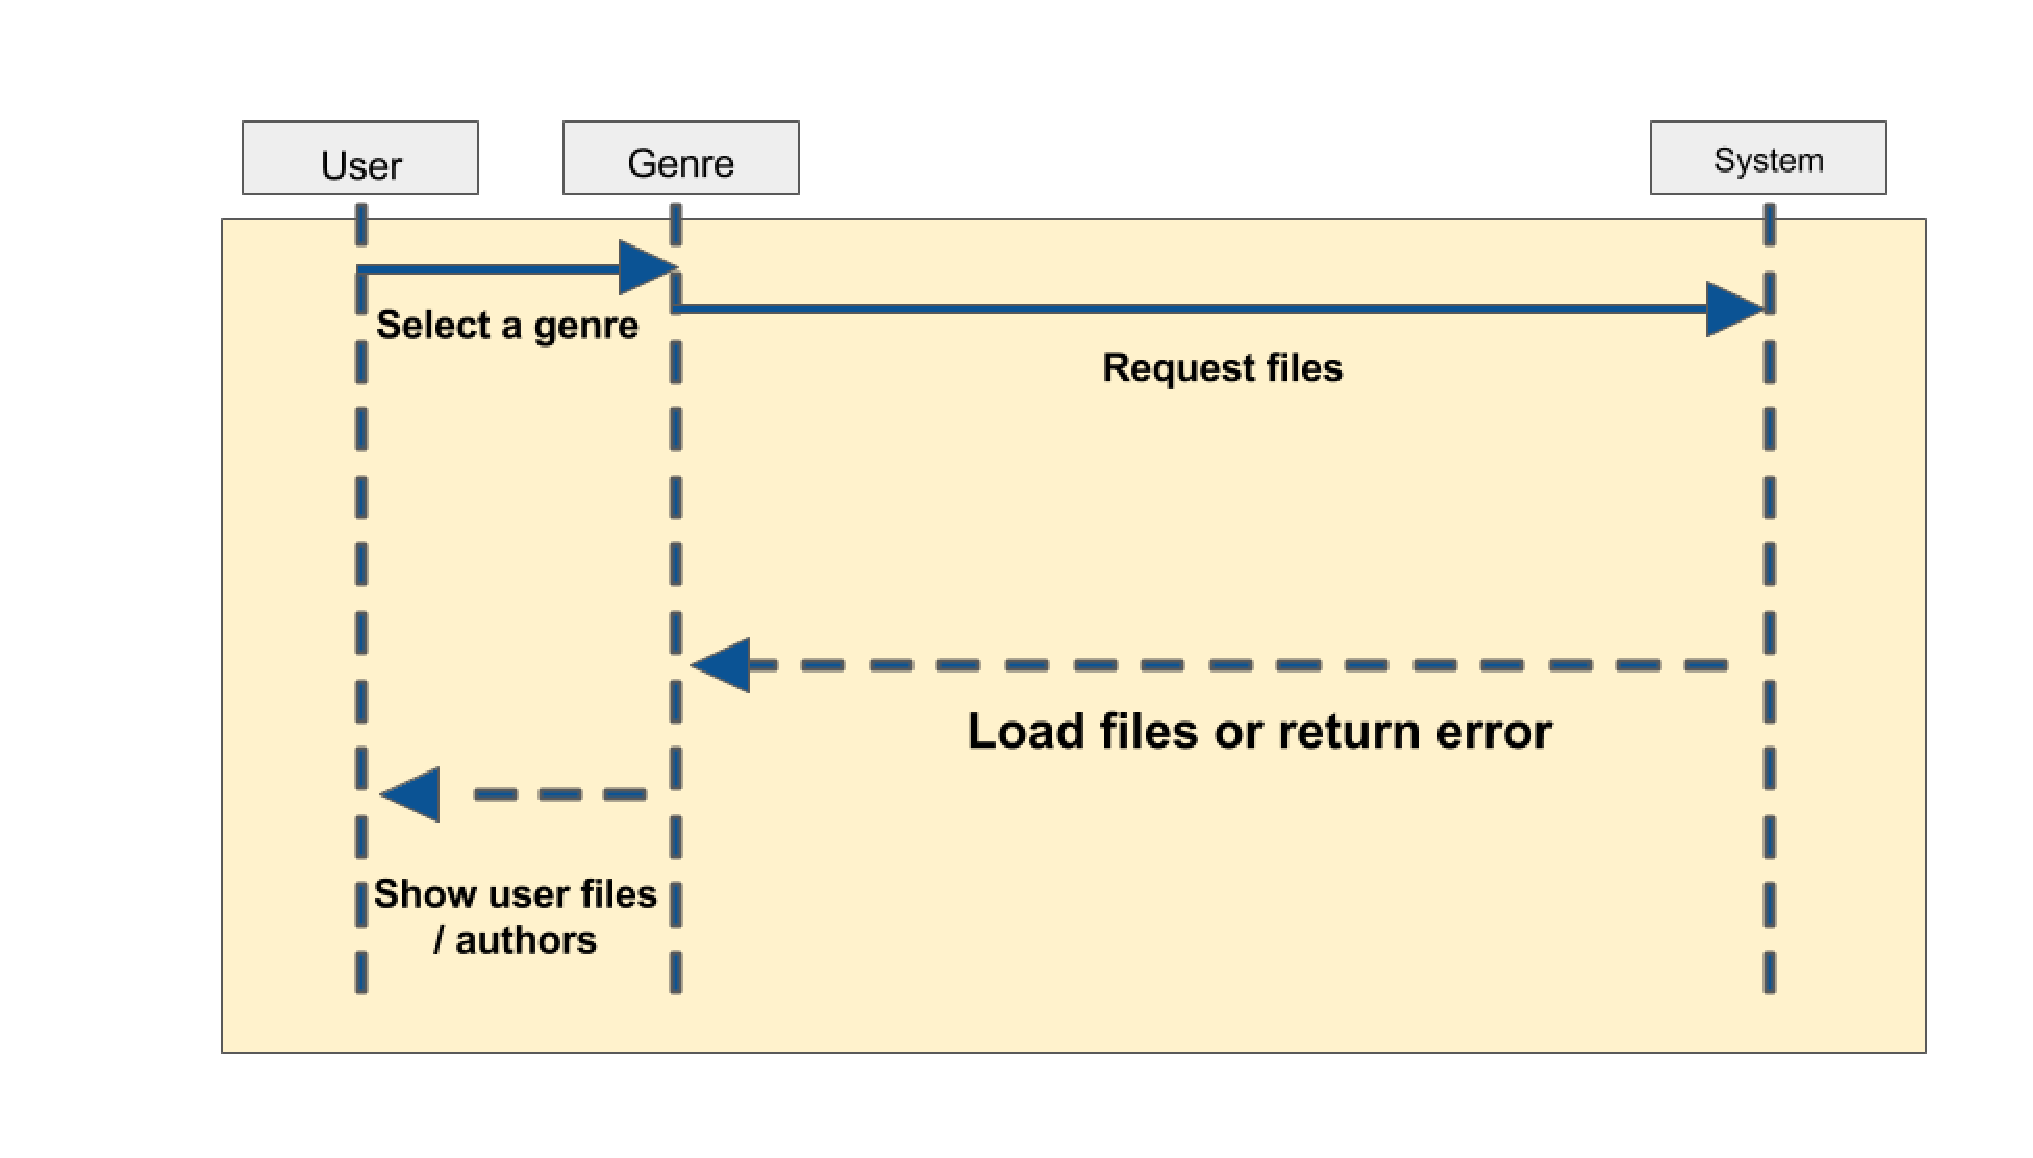
\includegraphics[scale=0.5]{Case3.eps}
\end{figure}

\newpage

\section{Meeting Report}

\subsection{This week's progress:}
Designed our project and defined specifications. We broke down the application into classes and identified the relationships between them, and defined the interactions our application will have with the existing word-rnn-tensorflow software and the operating system.

All team members have setup Python3.6, tensorflow, word-rnn-tensorflow, and PyGUI on their systems, we also have created our throwaway prototype of the GUI.

\subsection{Goals for next week:}
Develop a better understanding of python and the components that make up our project. Get started on implementing the GUI, as well as learning about file I/O, spawning child processes, and defining classes in Python.

\subsection{Contribution of team members:}
Jared Tence did not attend our Sunday meeting.
All attending team members worked on our assignment three.

\subsection{Were customers able to meet with the team:}
Yes. Team including customers met for our weekly Sunday meeting (2/4).




\end{document}
